\pdfoutput=1
\documentclass[a4paper,12pt,titlepage, twoside]{article}
\usepackage[english]{babel}
\usepackage[utf8]{inputenc}
\usepackage{amssymb,amsmath}
\usepackage{algorithm,algpseudocode}
\usepackage[title,titletoc]{appendix}
\usepackage{graphicx}
\usepackage{caption}
\usepackage{subcaption}
\numberwithin{figure}{section}
\usepackage{caption}


\begin{document}


% todo: compute Inception accuracy

\section{Introduction}
Estimated 80\% of the human data is in form of images or videos. There is a lot of useful information hidden, but it is still very complicated to gain it. Most of the information is still labeled manually by people, who make mistakes and are expensive. There is an incredible need for automated video processing in many branches of the industry. Being able to accurately detect and track vehicles can provide valuable data about transportation to governments. Reidentification and tracking objects over multiple cameras in real time can help reinforcement agencies to effectively fight crime. 

\subsection{Overview of methodology}
This thesis has been implemented for the company Good Vision s.r.o to be used in many South American cities for the police. The cameras are very wide angle and have been mounted directly to the street lamps.


\subsection{Contribution}
The author of this thesis implemented several modules for this project.

\begin{itemize}
\item The calibration of the camera and estimation of the vehicle position.

\item Detector and tracker of vehicles using classical methods

\item Semi-supervised data generator

\item Improving and extending and training deep learning detector and connecting it with a provided tracker.

\item Training a neural network for vehicles similarity

\item Testing and comparing results.


\end{itemize}

implementing of classical model detections.
using the facenet model for similarities.
Improving the ssd model.

\section{Related work}
state of the art

\section{Fish-eye camera model}

\begin{figure}[h]
\centering
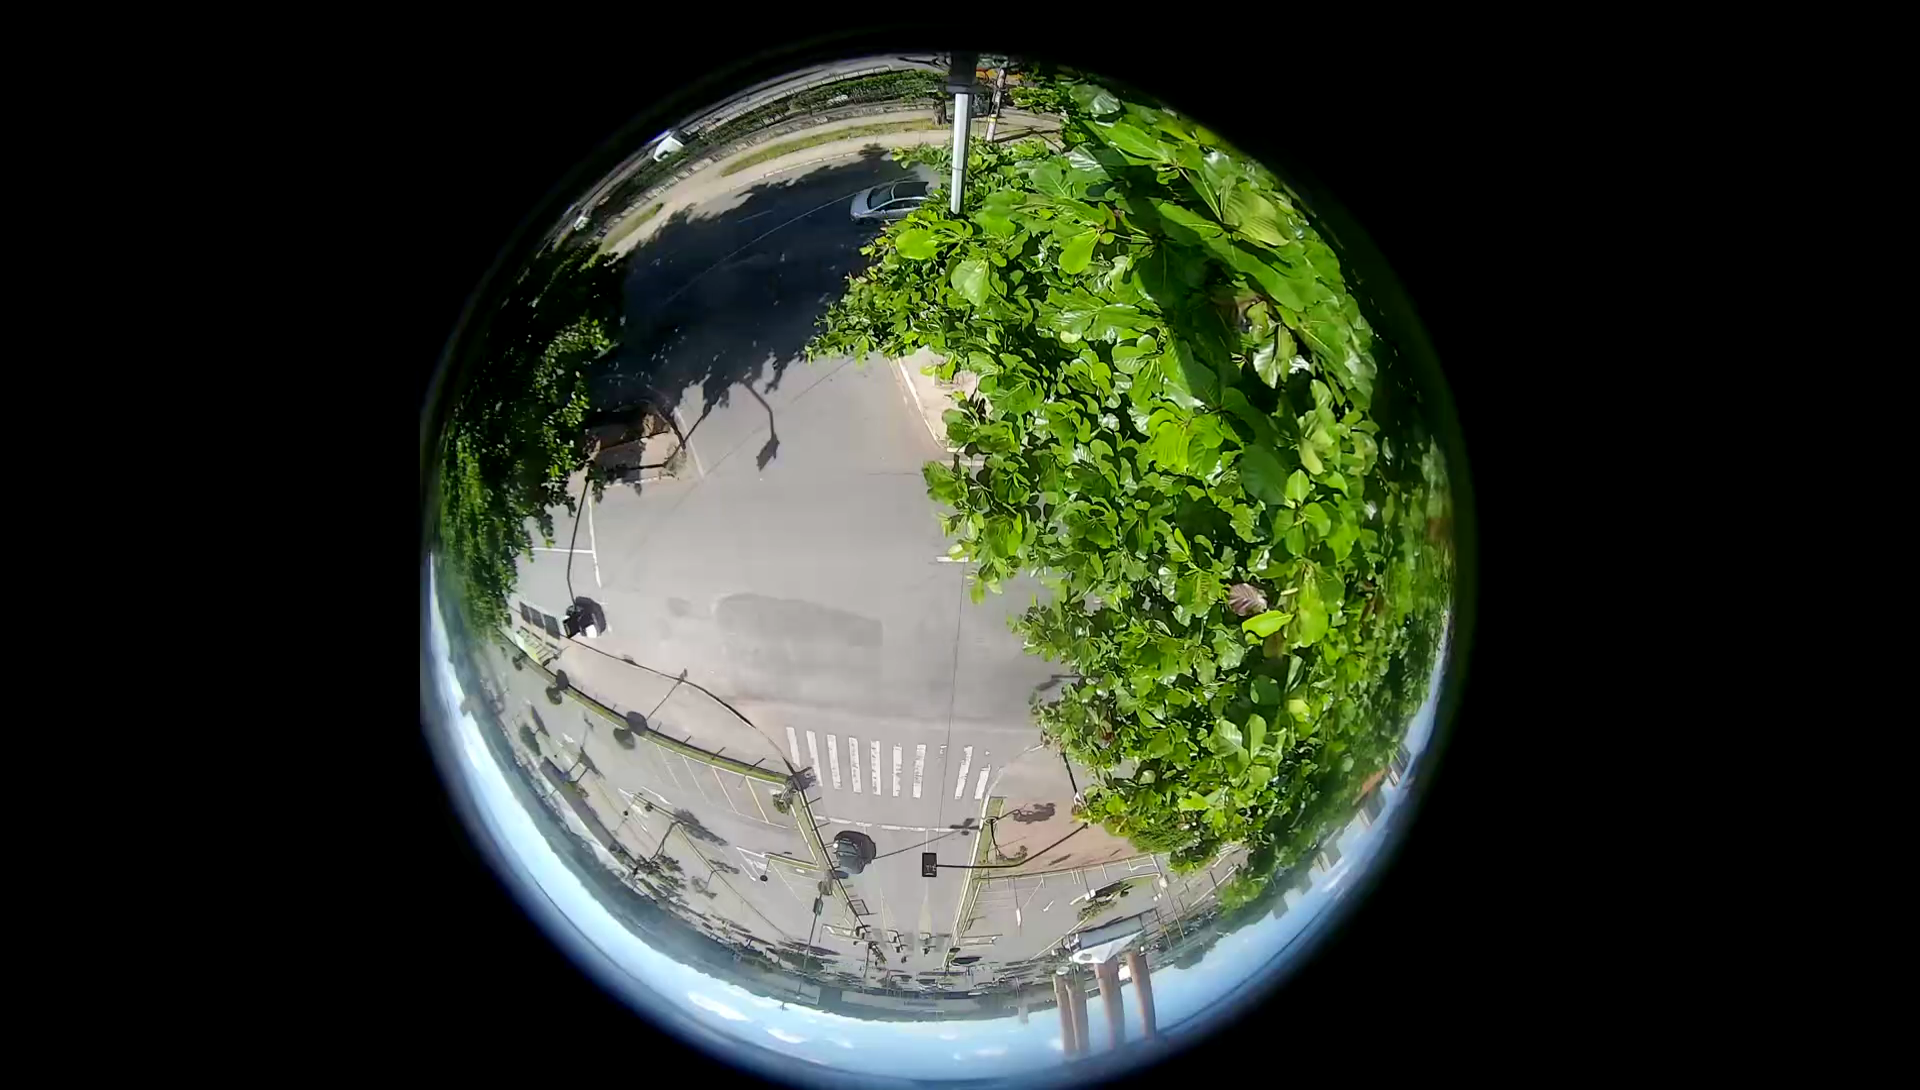
\includegraphics[width=1\linewidth]{fig/stream1.png}
\caption{Frame of the provided video}
\label{fig:stream1}
\end{figure}

For correct estimation of the position of detected objects, it is crucial to understand the camera optics and sensor. We need to find the transformations from the camera pixel position to the real world position. 

The cameras have been provided by the Brazilian party and no technical parameters are available. The model of the camera and it's parameters must be found. A set of improvised requested calibration images have been provided.

\subsection{Scene localization}
\label{sec:scene_localization}
Before we find the model of the optics, we need to compensate for another hardware error of the camera. As can be seen in the image \ref{fig:stream1}, the scene is shifted to the left down. It is not even circle, but rather an ellipse. This is due to manufacturing uncertainty and this error is different on each camera. Since this project will be easily scalable, and it is not convenient to measure and set the parameters manually, an universal algorithm for detecting ellipse has been introduced.

The algorithm is based on optimization. It takes an image as an input and produces parameters of the ellipse. From observation, the ellipse can only be either the horizontal major axis or the vertical major axis ellipse. The equation \ref{eq:ellipse} of the ellipse is rather unusual, but it allows faster cost function evaluation.

\begin{equation}
\label{eq:ellipse}
\frac{(x-s_x)^2}{a} + \frac{(y-s_y)^2}{1} = r^2
\end{equation}

Now we need to find the parameters $s_x, s_y, a, r$.

The original image $I$ of the size $H, W$ and channels $I_1, I_2, I_3$ is transformed to a mask $M$ of the same size by thresholding the total sum of channels on 8 bit scale is grater or equal to 1. \cite{lukacs1997real}

\begin{equation*}
M_{x,y} = \begin{cases}
1 & if \quad \sum_{i=1}^{3} I_{i,x,y} \geq 1 \\
0 & otherwise
\end{cases}
\end{equation*}

The mask $M$ represents the scene by the pixels with the value 1 and the background by the pixels with the value 0. 

We create an additional mask $E(s_x, s_y, a, r)$ of the ellipse as 

\begin{equation*}
E_{x,y}(s_x, s_y, a, r) = \begin{cases}
1 & if \frac{(x-s_x)^2}{a} + \frac{(y-s_y)^2}{1} \leq r^2 \\
0 & otherwise
\end{cases}
\end{equation*}

The cost function $C(M, E(s_x, s_y, a, r))$ penalizes the pixels that have been masked as the scene and lie outside the ellipse and the pixels, that have been masked as background and lie inside the ellipse.

\begin{equation}
C(M, s_x, s_y, a, r) = \sum_{x = 0}^{W-1} \sum_{y = 0}^{H-1} E_{x,y}(s_x, s_y, a, r) \cdot (1-M_{x,y}) + (1 - E_{x,y}(s_x, s_y, a, r)) \cdot M_{x,y}
\end{equation}

The algorithm could evaluate all combinations of parameters, but the number of searched parameters can be greatly reduced by searching in a coarse to to fine manner. 


\begin{verbatim}
x, y, a, r := initialize_params()
center_step, a_step, r_step := initialize_steps()

while(not imporoving):
    x_list := [x - center_step, x, x + center_step]
    y_list := [y - center_step, y, y + center_step]
    a_list := [a - a_step, a, a + a_step]
    r_list := [r - r_step, r, r + r_step]
    
    x, y, a, r := select_best(x_list, y_list, a_list, r_list)
    
    center_step := center_step / 2
    a_step := a_step / 2
    r_step := r_step / 2
    
return x, y, a, r
\end{verbatim}

This algorithm quickly finds the ellipse with very high precision. Furthermore the most expensive function, $select\_best$ can be highly parallelized.

\subsection{Camera model}

To correctly localize object from the camera, we need to know the transformations between real world coordinates $x^w, y^w, z^w$ and the projection on the captured frame $x^f, y^f$. After applying the algorithm from \ref{sec:scene_localization}, we know, where in the frame the scene is projected. First, we will consider the circle model and at the end we will apply the transformation to ellipse. 

Computing in the cartesian coordinates is not very useful for optics. Instead, the world coordinates are chosen to be spherical and the frame coordinates are chosen to be polar. The world coordinates are in respect to the camera. 
The transformations between the world cartesian coordinates $x^w, y^w, x^w$ and the world spherical coordinates $r^w, \theta^w, \phi^w$ are as follows:

\begin{figure}[h]
\centering
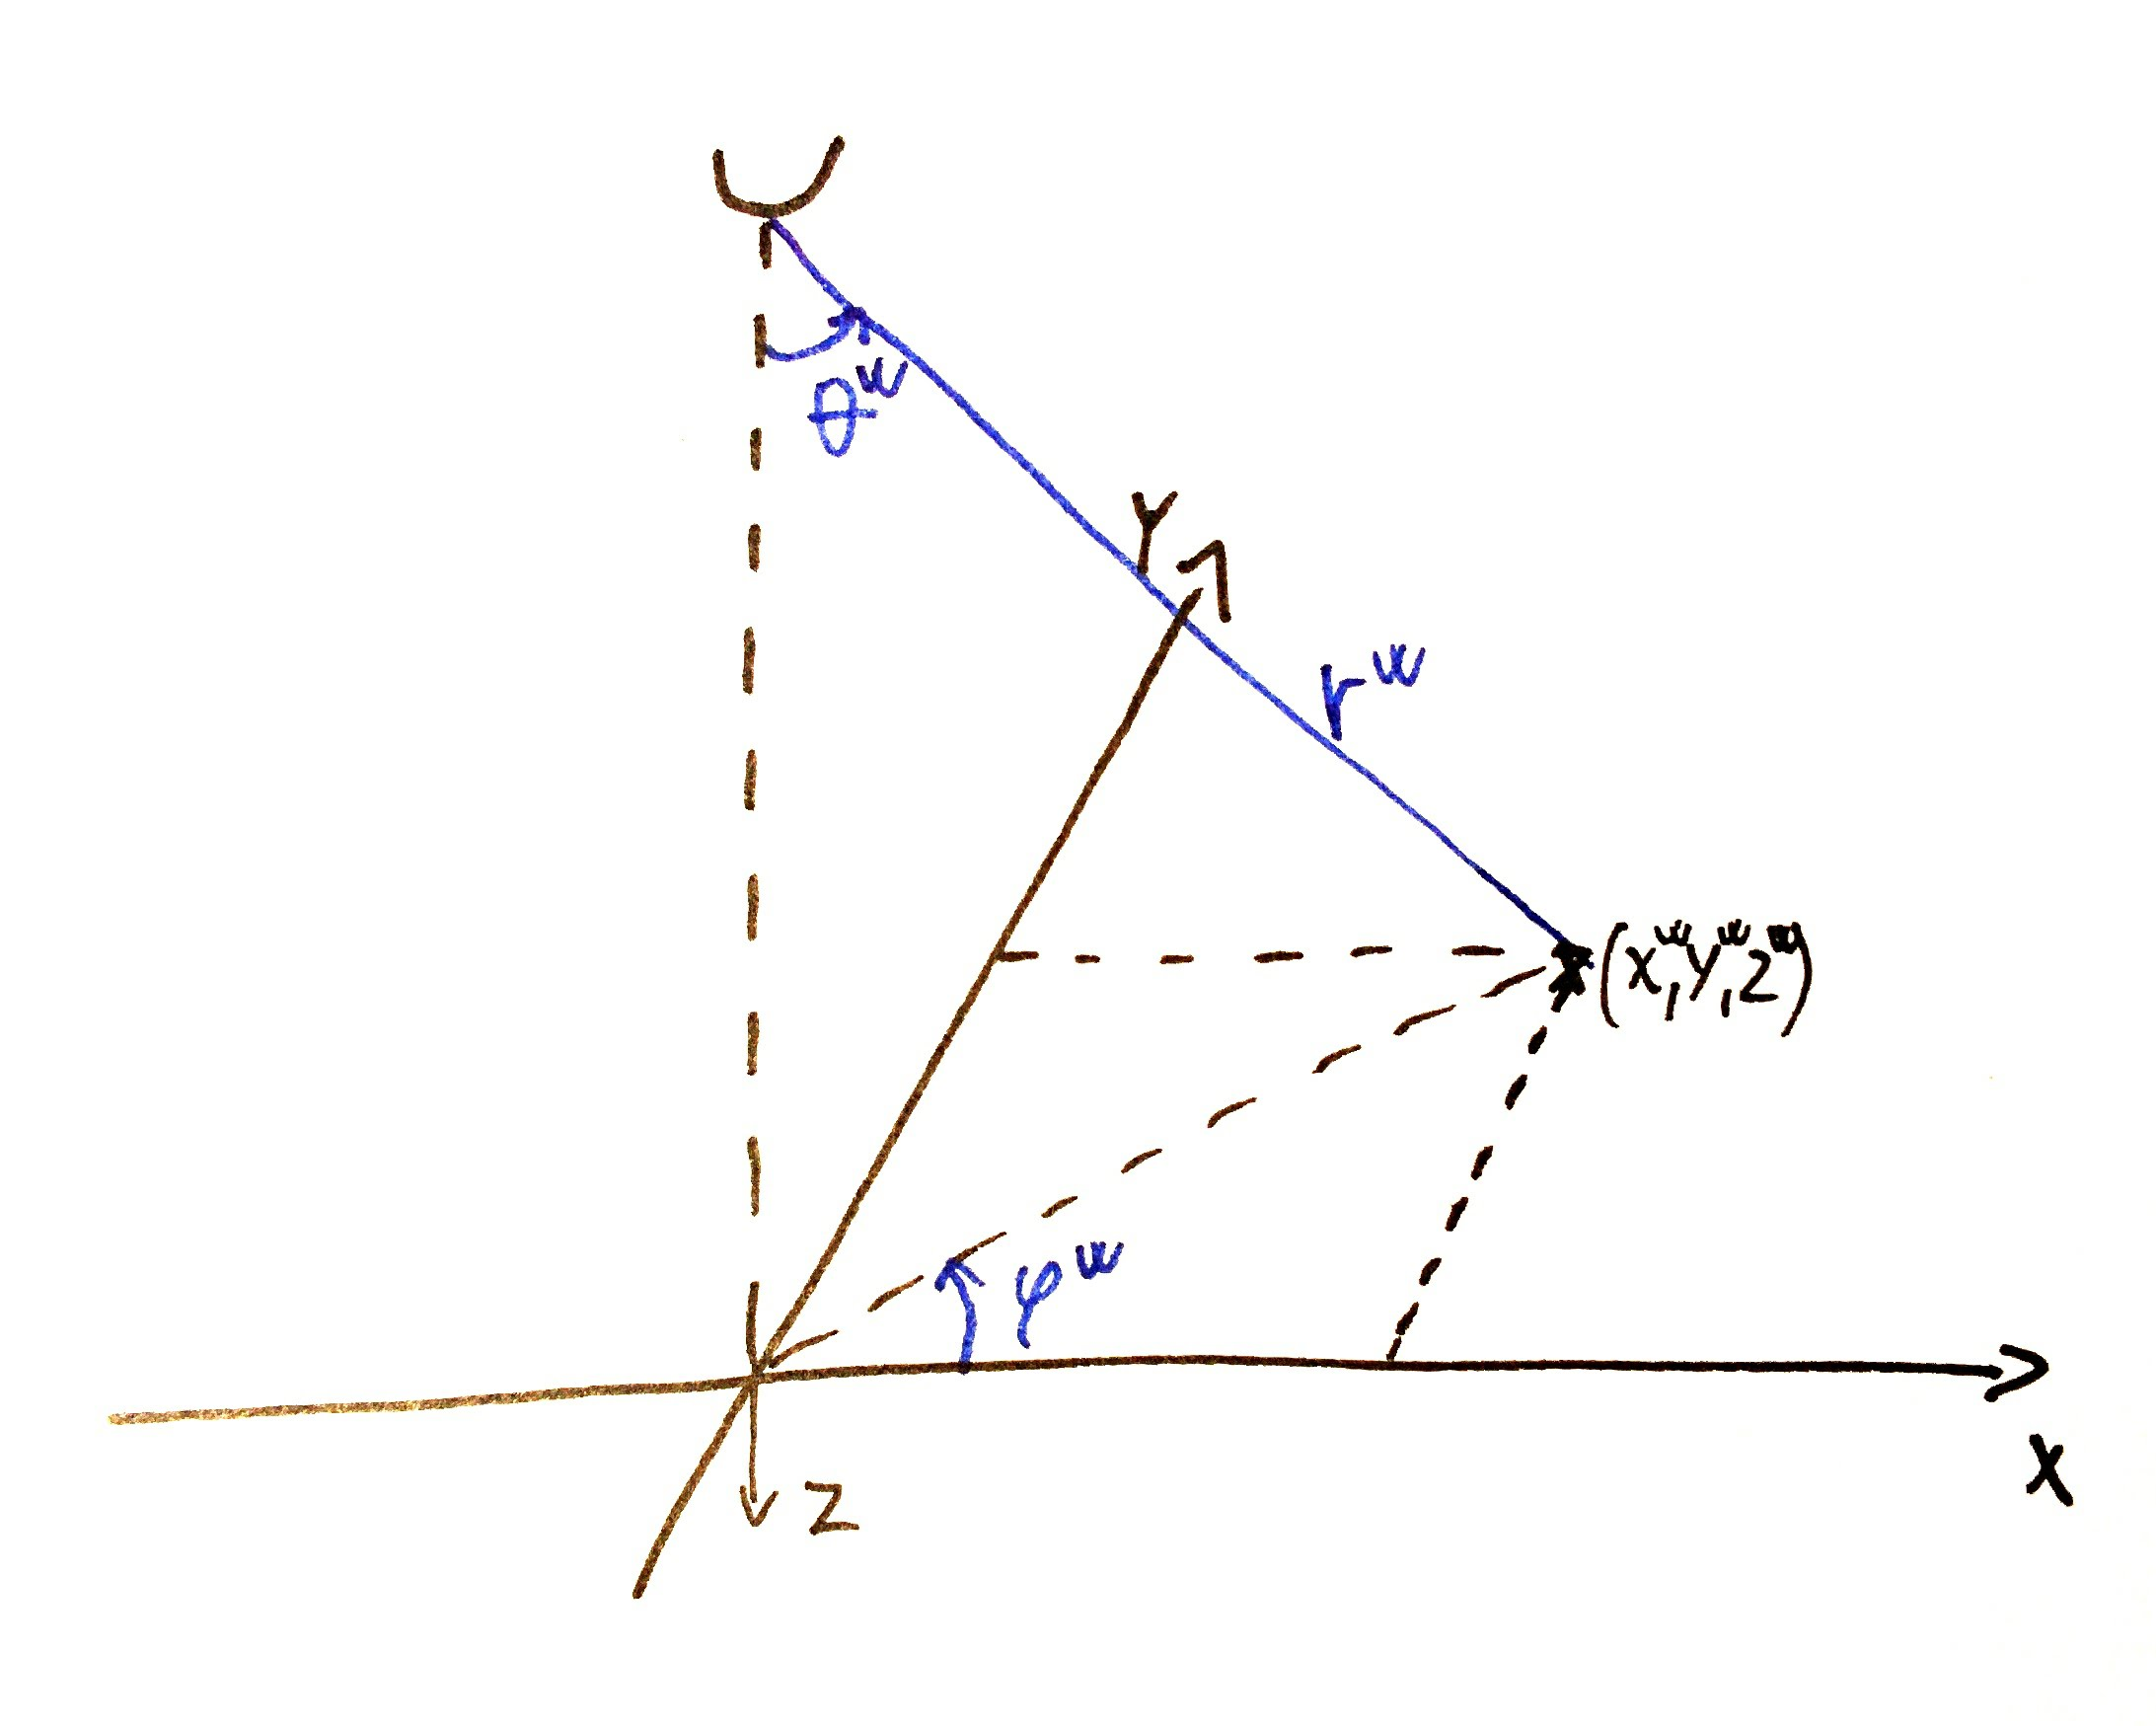
\includegraphics[width=1\linewidth]{fig/sphere.jpg}
\caption{The spherical coordinates of the world}
\label{fig:sphere}
\end{figure}


\begin{equation*}
\begin{aligned}[c]
x^w &= r^w \cdot cos(\theta^w) \cdot sin(\varphi^w) \\
y^w &= r^w \cdot cos(\theta^w) \cdot cos(\varphi^w) \\
z^w &= r^w \cdot sin(\theta^w) \\
\end{aligned}
\qquad,\qquad
\begin{aligned}[c]
r^w &= \sqrt{(x^w)^2 + (y^w)^2 + (z^w)^2} \\
\theta^w &= arcsin\Big(\frac{z^w}{r^w}\Big) \\
\varphi^w &= arctan\Big(\frac{y^w}{x^w}\Big) \\
\end{aligned}
\end{equation*}



The detected scene circle has the radius of $R$ pixels and the center at pixels $s_x, s_y$. The transformations between cartesian frame coordinates $x^f, y^f$ and the polar frame coordinates $r^f, \theta^f$ are:

\begin{equation*}
\begin{aligned}[c]
x^f &= s_x + R \cdot r^f \cdot cos(\varphi^f) \\
y^f &= s_y + R \cdot r^f \cdot sin(\varphi^f) \\
\end{aligned}
\qquad,\qquad
\begin{aligned}[c]
r^f &= \sqrt{(x^f - s_x)^2 + (y^f - s_y)^2} \\
\varphi^f &= arctan\big{(}\frac{y^f - s_y}{x^f - s_x}\big{)}
\end{aligned}
\end{equation*}

Next, we need to find the transformations between the world spherical coordinates $r^w, \theta^w, \phi^w$ and the frame polar coordinates $r^f, \theta^f$, but there are some nice properties:

\begin{itemize}
\item The $\varphi$ are the same, i.e. $\varphi^w = \varphi^f$.
\item The transformations do not depend on $r^w$. The projection depends only on the direction, not on the distance from camera.
\end{itemize}

With this knowledge, we need only to find the transformation of $\theta^w$ and $r^f$. We need to find a function $f$, such as 
\begin{equation}
\begin{aligned}
\theta^w &= f(r^f) \\
r^f &= f^{-1}(\theta^w). \\
\end{aligned}
\end{equation}

There are many models for finding $f$. 

\begin{itemize}
\item The linear model: $f(r^f) = FOV \cdot r^f$
\item The tangent model: $f(r^f) = FOV \cdot \tan(r^f)$
\item The sinus model: $f(r^f) = FOV \cdot \sin(r^f)$
\end{itemize}

With each model, we need to find the one parameter $FOV$, which is the field of view of the camera.

There was no access to the cameras, so the standard calibration using mesh could not be used. Instead, a set of marks was provided as shown in the picture. These marks are exactly 2 meters apart and are enough to estimate the function $f(r^f)$.

\begin{figure}[h!]
\centering
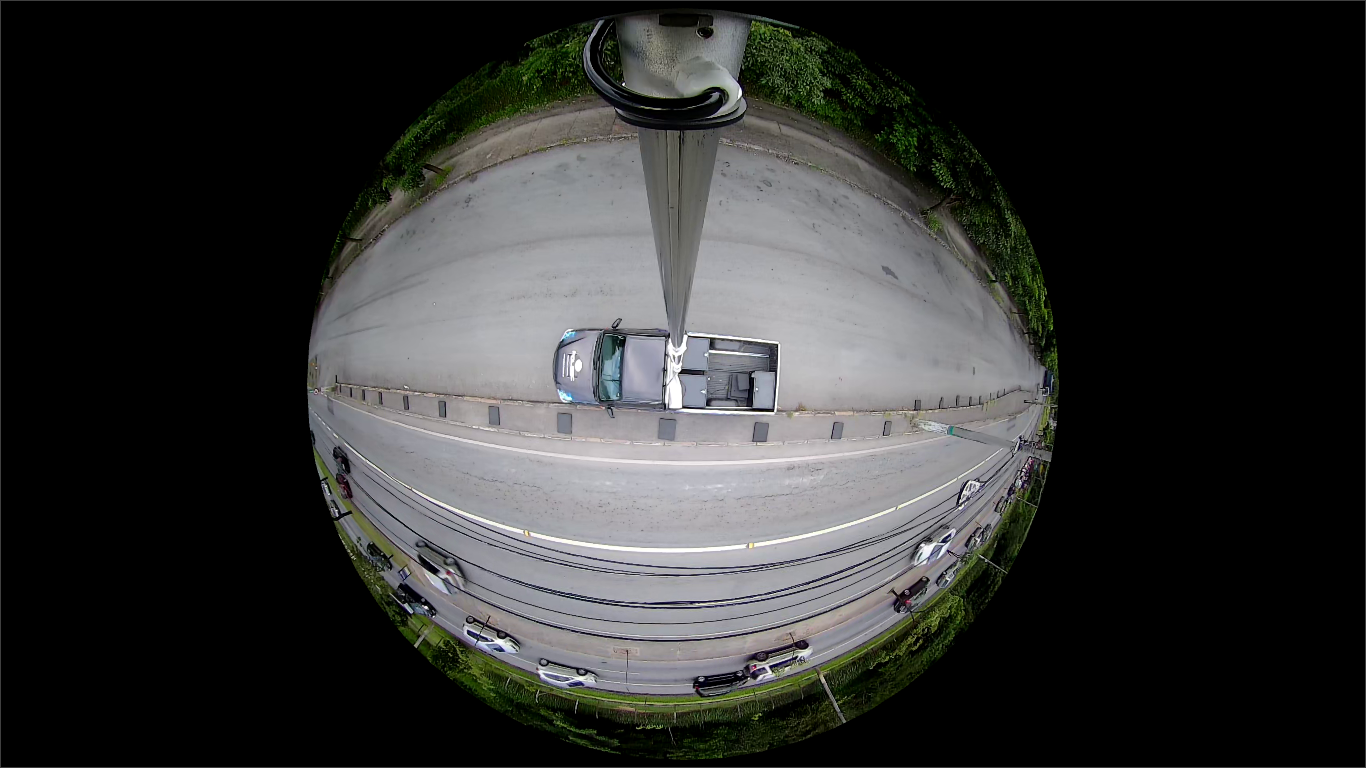
\includegraphics[width=1\linewidth]{fig/calibration.png}
\caption{The provided calibration data}
\label{fig:calibration}
\end{figure}


\subsubsection{Linear model}

This is the simplest one. The real world angle is proportional to the distance from the center on the image. 

\begin{equation}
\theta^w = f(r^f) = FOV \cdot r^f
\end{equation}

Fitting of the model is shown in the fig.\ref{fig:linear_model}

\begin{figure}[h!]
\centering
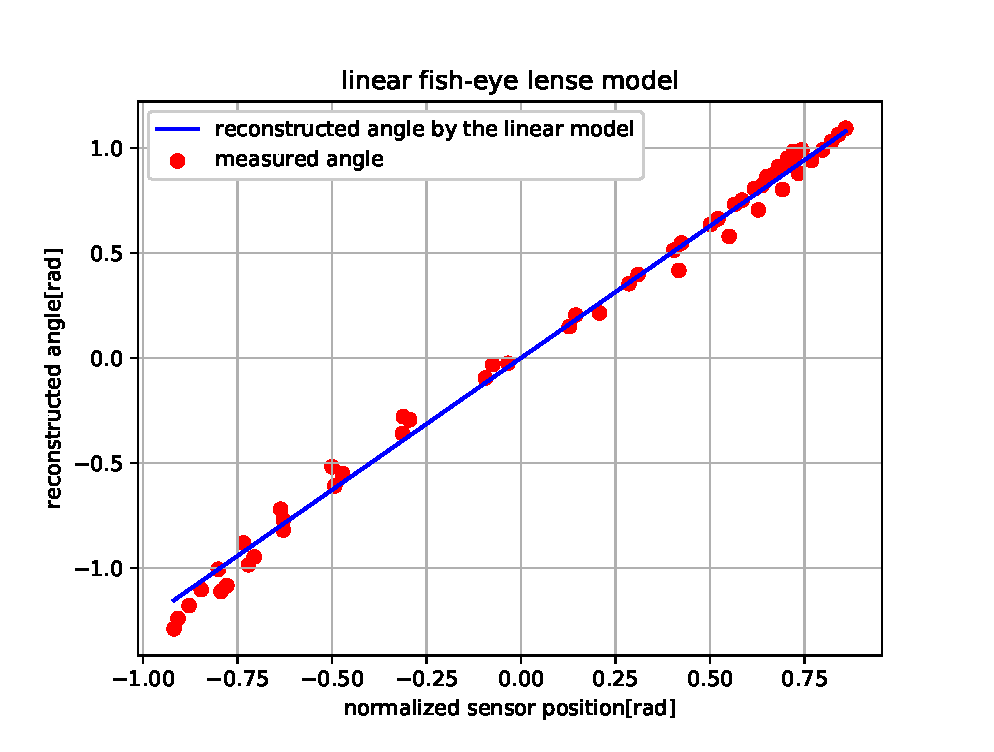
\includegraphics[width=1\linewidth]{fig/linear_model3.eps}
\caption{The linear model of the lens}
\label{fig:linear_model}
\end{figure}

The linear model somehow estimates the real one, but not that well.

\subsubsection{Tangent model}

This is a more complicated model, which is based on the pinhole camera model.

\begin{equation}
\theta^w = f(r^f) = \theta^w \cdot FOV,
\end{equation}

Fitting of the model is shown in the fig.\ref{fig:linear_model}

\begin{figure}[h!]
\centering
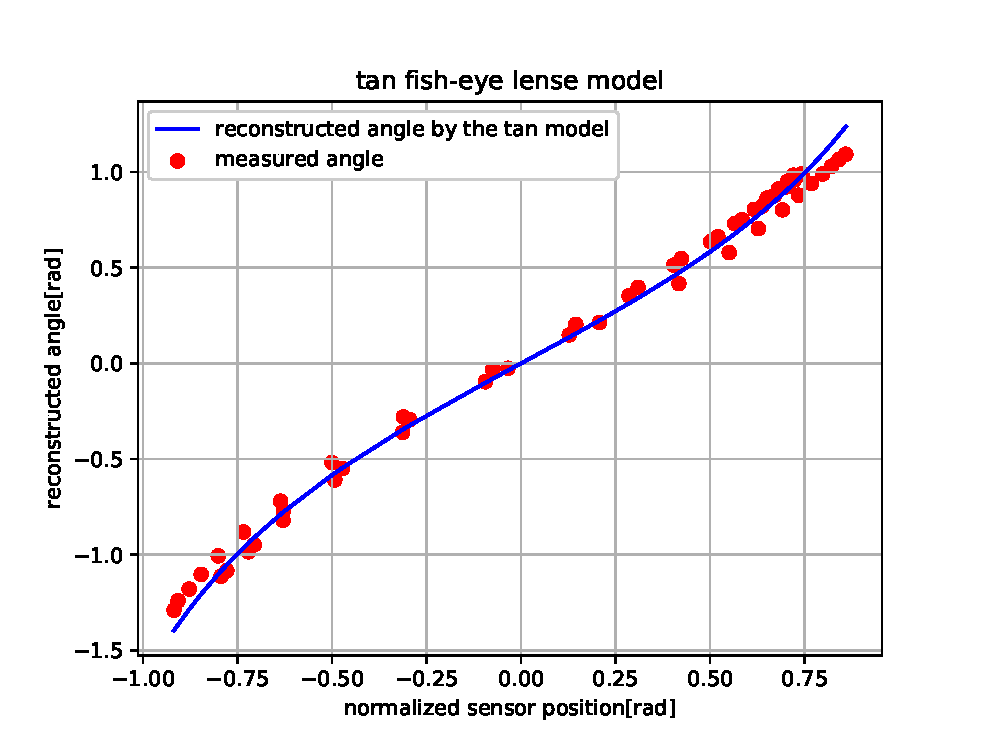
\includegraphics[width=1\linewidth]{fig/tan_model2.eps}
\caption{The linear model of the lens}
\label{fig:linear_model}
\end{figure}

This model represents the camera optics much better and was chosen to be the final one.

\subsection{Real world coordinates}

There is many ways how to represent real world for representing the car in the city. The most ovious one would be represent the position by longitude, latitude and elevation. This is exact, but not very practical. Since the distances between same circles of latitude and longitude are different, this would need more complicated transformations and there is a simple model. 

Since we care only about only one city, one camera will be the frame of reference.








\section{Detection Evaluation}
For training a neural network, it is important to have some means of evaluating it, so we can compare models. We need to have some algorithm of evaluating the detections on an images against the ground truth. With the detection problem, this is more complicated, than the classification problem.

\subsection{Classification evaluation}

The classification problem is easier than the detection problem. Given the image, predict a class, which is picked from previously known set of classes. The classifier can also return the probability distribution, in which case, the predicted class is the one with the highest probability. There are several metrics for measuring accuracy.

\subsubsection{top 1 accuracy}

The classifier returns the predicted class. If the class matches with the ground truth, the accuracy is 1, otherwise it is 0.

\subsection{top 5 accuracy}

Another evaluation is the top 5 accuracy, used for example in imagenet \cite{imagenet} competition. In this evaluation, the detector predicts 5 classes and if the ground truth is among them, it returns 1, otherwise 0. 

\subsection{Mean average precision.}
Mean average precision (mAP) is the most used metrics for object detection problem. The advantage is, that it does not depend on the selected confidence threshold, but only on the IoU threshold. This metrics is not constrained only for object detection problems in vision, but can be used for all detection problems. 

The algorithm for computing mAP runs for all thresholds. Given an arbitrary threshold, the predicted bounding boxes are those, whose confidence exceeds it. If there is a high IoU of a ground truth box and some predicted bounding boxes having the same class, the predicted box with the highest confidence is matched and considered true positive($TP$) and no other box can be matched with the ground truth bounding box. If a predicted bounding box is not matched with any ground truth bounding boxes, it is considered false positive($FP$). If a ground truth bounding box is not matched with any predicted bounding box, it is considered a false negative($FN$).

Precision($P$) corresponds to what portion of ground truth boxes have been matched. With lowering the threshold, it can only increase, since more ground truth bounding boxes will be matched.
\begin{equation}
P = \frac{TP}{TP + FP}
\end{equation}

Recall($R$) corresponds to what portion of predicted bounding boxes have been matched. 
\begin{equation}
R = \frac{TP}{TP + FN}
\end{equation}

The precision-recall curve in the Fig.\ref{fig:precision-recall} shows the dependency of precision and recall. The higher the precision, the lower the recall. The area below the curve is called average precision($AP$) and the mean over all classes is called mean average precision($mAP$).

\begin{equation}
mAP = \frac{1}{|C|} \sum_{c \in C} AP_c
\end{equation}

where $C$ is the set of classes.

\begin{figure}[H]
\centering
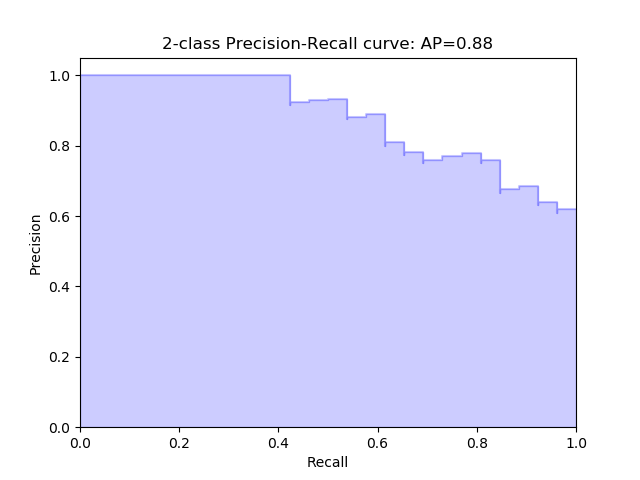
\includegraphics[width=1\linewidth]{fig/precision-recall.png}
\caption{Example of precision-recall curve}
\label{fig:precision-recall}
\end{figure}




\section{Classical detector}
The final will be easily scalable and a particular system architecture has been explored. If the detections and tracking were computed on-board of the cameras, that would help greatly. There would be much less communication needed. Instead of transferring whole video streams, only some meta-data would be sent. That would include: 

\begin{itemize}
\item Time stamps of a frames.
\item Locations of objects and their classes.
\item Some description vector of the detections.
\item Detections clustered to tracks.
\end{itemize}

This system could be greatly distributed sending packets of information among only the cameras that the information is relevant to.

However this has some downfalls, mainly in computational manner. Each camera would have to be equipped either with a capable computational unit. The detections, tracking and similarities would all have to be computed onboard. Since it is not possible to have a GPU in every lamp for many reasons, for example it is a very wet environment, usage of neural networks would not be possible and some classical detection and tracking methods running on CPU have been explored and developed.



\subsection{Background subtraction}
\label{sec:bgs}

Probably the best classical detection methods from static videos, that can be computed in real time on limited hardware, are based on the background subtraction algorithm \cite{...}. The main idea is creating a model of the scene without the objects that we want to detect and then subtracting the current frame and by thresholding determine, where the vehicles are. This simple approach does not work very well and some improvements need to be made. 

For the background subtraction procedure, a model of the background has to be found. For our purposes we need to know, how the road looks like without any vehicles and people. This can't be done by simply waiting for such a case, because the traffic is usually quite high. Instead, we need to figure out the background from more multiple frames. 

The algorithm has been implemented in opencv \cite{opencv}. The background is generally created by the mean over several images \cite{bs1, bs2}. It is also updated with each new frame as a weighted sum. The background looks like a photo with a long exposition and the lane, where vehicles drive has a colored lines as shown in the figure \ref{fig:cut_mean}. When computed the difference from a video frame to such a background model, as shown in the figure \ref{fig:threshold_mean}, the places, where usually cars drive, can have high values. This can be bad for creating a mask by thresholding, because a higher thresholding constant has to be set.

\begin{figure}
    \begin{subfigure}[Sample1]{0.5\linewidth}
        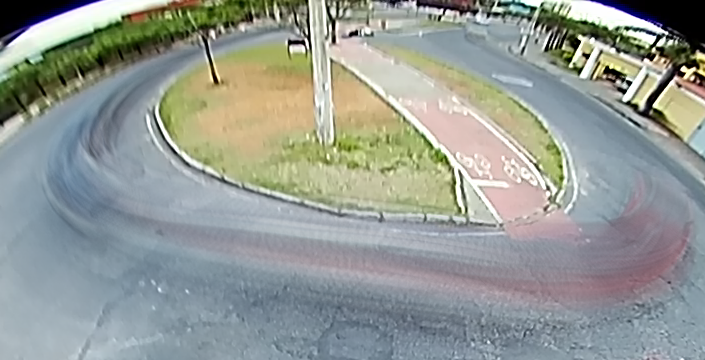
\includegraphics[height=37mm]{fig/background_mean_crop.png}
        \caption{Mean model}
        \label{fig:cut_mean}
    \end{subfigure}
    \qquad
    \begin{subfigure}[Sample1]{0.5\linewidth}    
        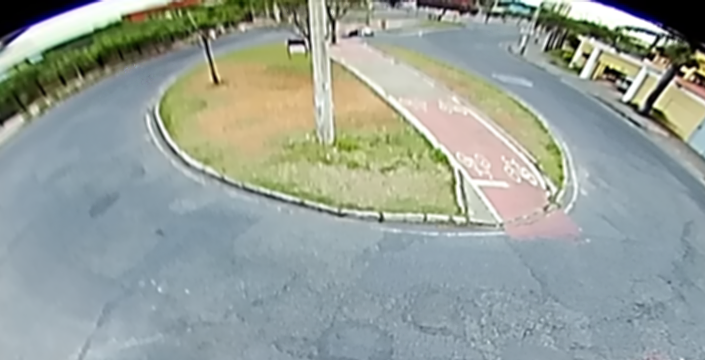
\includegraphics[height=37mm]{fig/background_med_crop.png}  
        \caption{Median model}
        \label{fig:cut_med}  
    \end{subfigure} 
    \caption{Background model created by the mean and the median approach.}
\end{figure}

The background model changes with every new frame. In the first iteration, the background $B_0$ is just the first frame $F_0$. The background in next iteration is just the weighted sum of the  current frame and the background model in the previous iteration.

\begin{equation}
B_n = \alpha \cdot F_n + (1 - \alpha) \cdot B_{n-1}
\end{equation}

This algorithm is very fast and can be highly parallelized and computed on graphics cards. The picture having $N$  pixels, the complexity of this standard background subtraction algorithm is  $O(N)$.



\begin{figure}
    \begin{subfigure}[Sample1]{0.5\linewidth}
        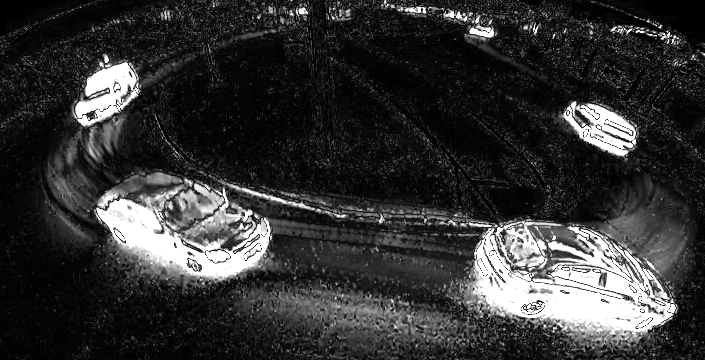
\includegraphics[height=37mm]{fig/threshold_mean_crop.png}
        \caption{Mean}
        \label{fig:threshold_mean}
    \end{subfigure}
    \qquad
    \begin{subfigure}[Sample1]{0.5\linewidth}    
        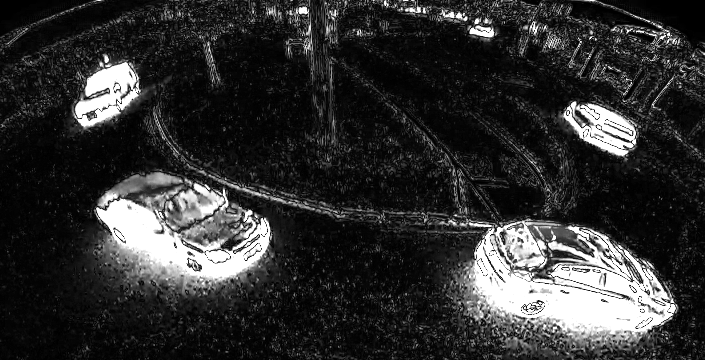
\includegraphics[height=37mm]{fig/threshold_med_crop.png}
        \caption{Median}
        \label{fig:threshold_med}    
    \end{subfigure} 
    \caption{The difference between the frame and a background shown in a gray-scale.}
\end{figure}

A new approach has been introduced, which greatly improves the quality of current background subtraction methods. A simple change of taking the median instead of the mean at each pixel position gives much better estimation of the background. The algorithm keeps a queue of $K$ images in a memory and with each incoming frame it puts it in the database and for each pixel it computes a median from the queue. This algorithm can be implemented with the complexity $O(N \cdot log(K))$, if we insert each pixel from an incoming frame to a sorted structure. In reality, for small $K$ this would slow the algorithm, because in opencv and numpy there is a great support for working with the whole images. This approach is simply compute the median over all the images from the queue. The complexity is $O(N \cdot K \cdot log(k)).$ The $K$ has been set to 35. The histogram of a particular pixel position over the queue is show in the figure \ref{fig:pixel_hist}.


This turns out to work much better, but still has it's limits. If the traffic is very high and vehicles occupy in average more than half of the ground, the background model will fail, but mean approach would fail as well. 

\begin{figure}[h]
\centering
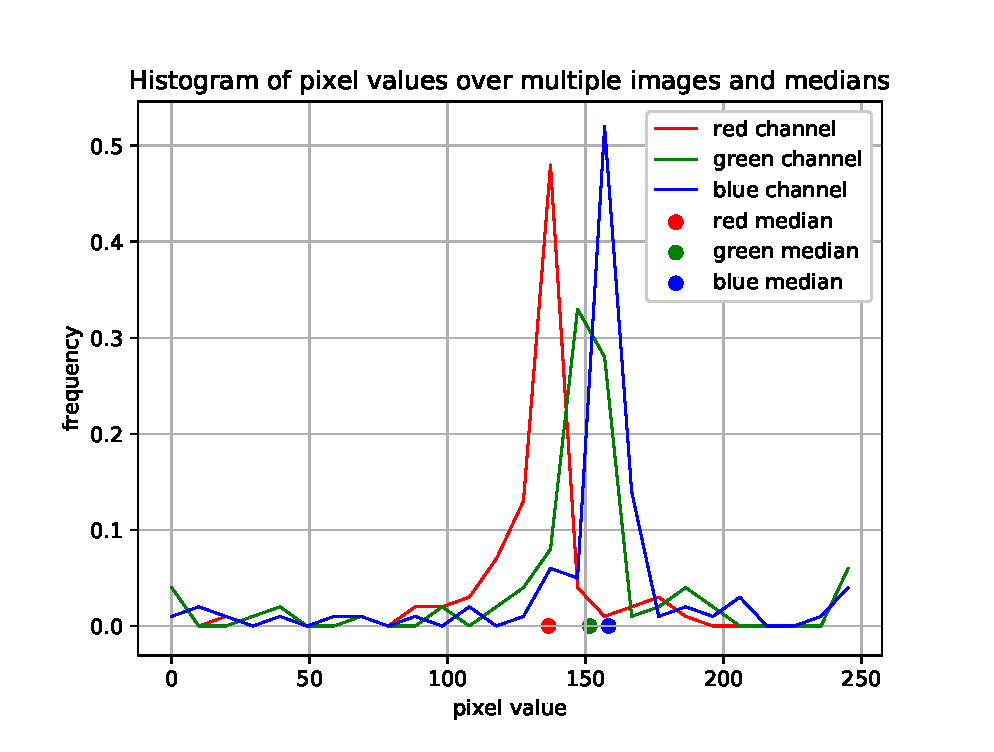
\includegraphics[width=1\linewidth]{fig/pixel_hist.eps}
\caption{The histogram of a particular pixel over 100 images with computed medians}
\label{fig:pixel_hist}
\end{figure}

Some more complicated models based on unsupervised learning, such as clustering or taking the most frequent bin from histogram for each pixel position could be used, but they would be computationally too complex and would not be practical for realtime video.

The difference between background model and the current frame is very noisy and some filtration has to be made. Before subtraction, the background and the frame has been filtrated with a gaussian filter with the size 3x3 for smoothing. This compensates for the camera vibrations. Then smoothed again with the filter 11x11. This serves as an apriori probability. The idea is, that if there are big differences in the neighboring area, it is a higher probability of the pixel belonging to the car. This also helps to detect gray and black cars, which have similar color to the road. Another advantage is, that this greatly reduces noise and helps to detect vehicles as whole.

This differential image is thresholded and a mask is obtained as shown in the figure \ref{fig:mask_area}. Each blob is presented with a contour and they are thresholded once more by the area. The resulted blobs become detections and a bounding box is created.

\begin{figure}
    \begin{subfigure}[Sample1]{0.5\linewidth}
    	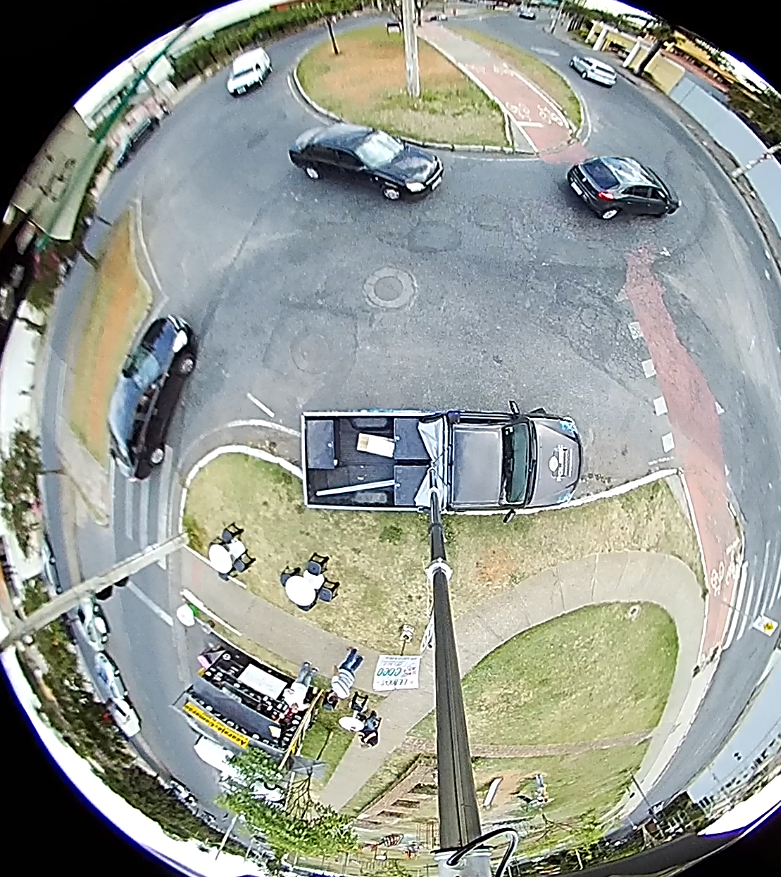
\includegraphics[height=85mm]{fig/frame_cropped.png} 
        \caption{A frame for detection}
        \label{fig:frame_for_detection}   
    \end{subfigure}
    \qquad
    \begin{subfigure}[Sample1]{0.5\linewidth} 
    	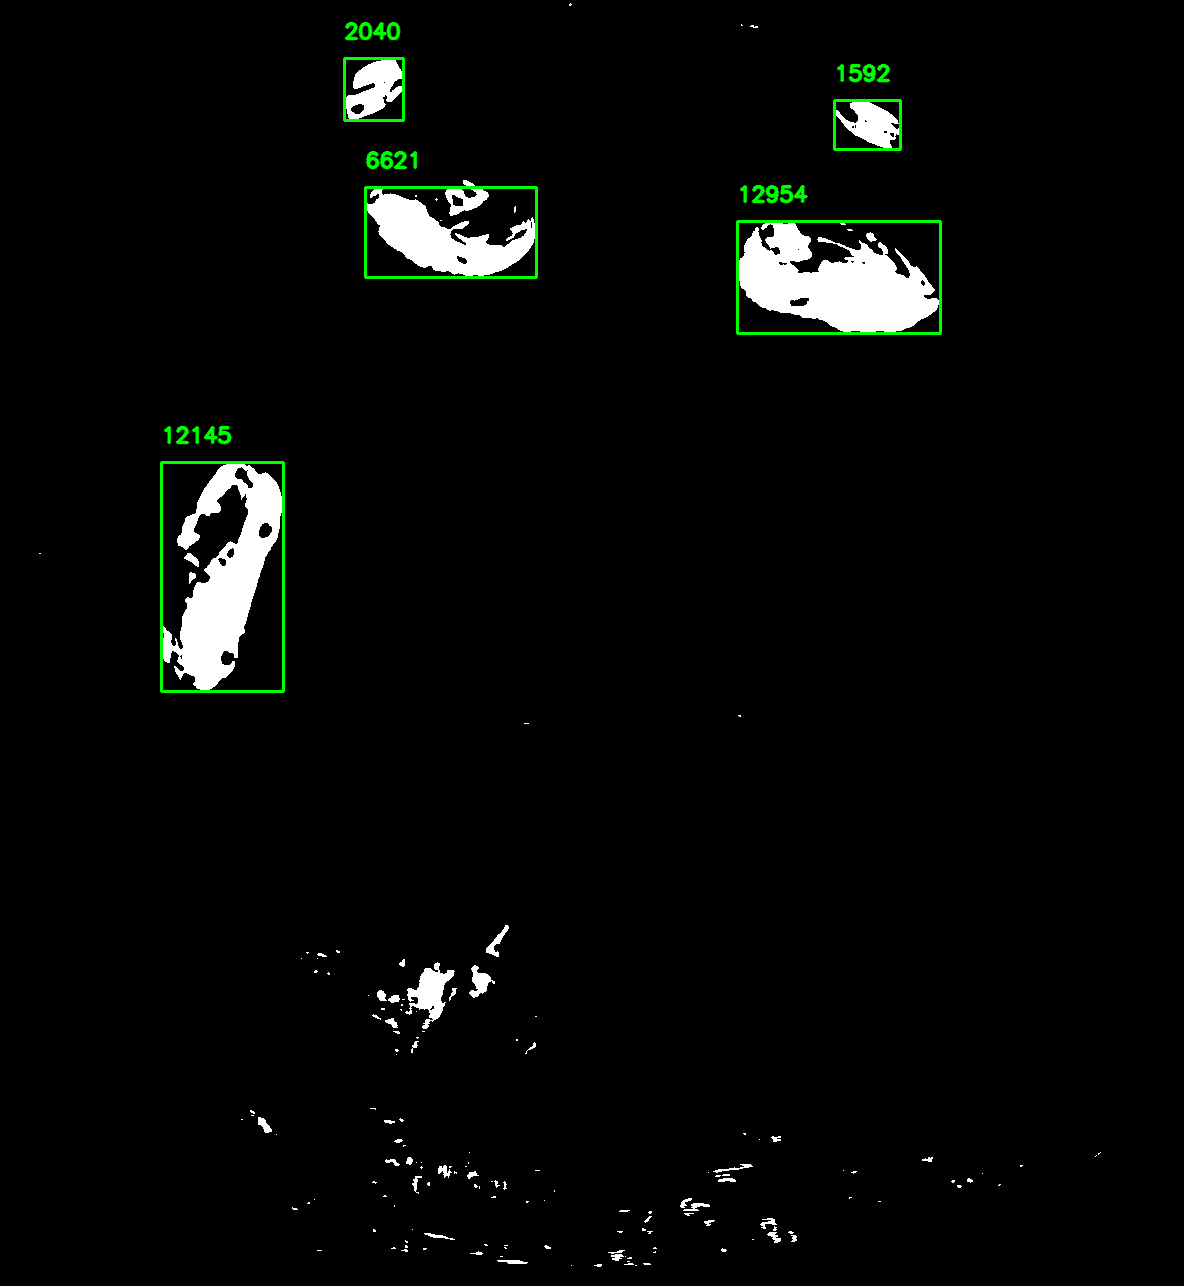
\includegraphics[height=85mm]{fig/mask_area.png}
        \caption{The detections and areas of contours.}   
        \label{fig:mask_area}
    \end{subfigure} 
    \caption{The background subtraction detection algorithm.}
\end{figure}

The background must be continuously adapting to the scene, but the rate of adapting is crucial. If the background is changing too slowly, it will not work very well with changes of lightning from coming clouds, etc. If the background adapts too fast, it will start to contain cars, that stop at the cross section and when the cars leave, this will become a new false detection. From experiments, there is no optimal adapting rate and it depends on the scene, weather and even then these problems will not completely disappear. One small advantage is filtering detections while adapting background.

Background subtraction is a very fast detection algorithm and when having perfect conditions, it is very accurate and The bounding boxes are more precise than most deep learning approaches.

Unfortunately it has many downsides. 

\begin{itemize}
\item Moving trees and their shadows create false positives.
\item Overlapping vehicles are detected as only one.
\item It works bad in high traffic, because it can't create a correct background model.
\item It is very sensitive to changes of lightning, such as moving clouds.
\item It is very sensitive to correct setting of hyper-parameters.
\end{itemize}

Most of these points relate to changing background. Especially if the scene is partially cloudy and the lightning changes a lot, the background model needs to adapt quickly. On the other hand, if in the scene is a traffic light, cars spend a lot of time on one spot and could be incorporated to the background model. Not only the car will not be detected, but a false positive will be detected when the car leaves.

For these problems, background subtraction alone can't be used as a good detector, but on perfect scenes  it can be very useful for collecting high quality training data for neural networks detectors, as described in the section \ref{...}.

\subsection{Optical Flow}

The detections have been described in section \ref{sec:bgs}. Having only the detections for each frame does not give us that much information. We need to connect these detections to a track, which is a sequence of detections over the frames, in which the object appears in the scene.

A custom set of algorithms has been implemented in opencv\cite{opencv} for extending the background subtraction algorithm. Optical flow \cite{optical-flow} is used for a motion estimation. It estimates a motion vector to each 


Harris corner features
shi-thomasi


is not used over the whole image, since that would be too expensive. Instead, each detection is extended for a one optical flow point. In the next frame, this point will move with the object. This extends the detector for object tracking and partially solves the problem of two overlapping vehicles. If two vehicles drive close to each other, background subtraction would start to treat them as one object. This improved model will detect this situation and keep the bounding boxes on the different vehicles. 

There is a set of rules, but these are the main ones:
\begin{itemize}
	\item If an optical flow point is outside the background subtraction mask, it becomes a 'zombie'.
	\item If a background subtraction detection is without an optical flow point and there is no 'zombie' in the detection, optical flow point is created in the middle of the bounding box. 
	\item If a zombie is not recovered in 10 frames, it disappears. 
	\item If there are more optical flow points in one background subtraction detection, the bounding boxes continue movement with a low pass filter.
	\item The optical flow points are forced to the middle of the bounding box. This solves the problem of the detection being put on the front of the car while coming and due to noise later being outside the bounding box, when the vehicle is viewed from a side. 
\end{itemize}

These improvements work surprisingly well and solve the tracking problem to some extent. If vehicles overlap completely, this approach will fail, but so will most of the other ones. 


% corello








\bibliographystyle{plain}
\bibliography{ref}{}
\cleardoublepage
\clearpage

\end{document}